\section{Theorie}
Ein Laser ist eine Apparatur, welche monochromatisches Licht in hoher Intensität und Kohärenz emmittiert. Um ein solches Licht 
zu erzeugen, bedarf es drei grundlegenden Kompoenenten welche an dieser Stelle näher beleuchtet werden sollen.
Ganz allgmein wird ein aktives Lasermedium, ein Resonator sowie eine Pumpquelle für den erfolgreichen Betrieb eines Lasers benötigt.

Das Lasermedium wird durch die Ausnutzung des Effektes der simulierten Emmission so manipuliert, dass das durch das Lasermedium transmittierte Licht
eine Verstärkung erfährt. Um diesen Effekt verstehen zu können, wird das Lasermedium als zwei Niveau System betrachtet.
Dieses System kann durch Absorption angeregt werden, indem es die Energie eines Photons aufnimmt. In diesem Zustand gibt es
zwei Prozesse mit derer das System, die Energie wieder abgehen kann. Der erste Prozess ist die stimulierte Emission, welcher hier nicht
näher betrachtet wird. Der zweite Prozess ist die stimulierte Emission, hier wird das System unter Einfall eines weiteren Photons in den Grundzustand übergehen. Jedoch wird
hierbei ein weiteres Photon mit den gleichen Eigenschaften des einfallenden Photons erzeugt.

\begin{figure}
  \centering
  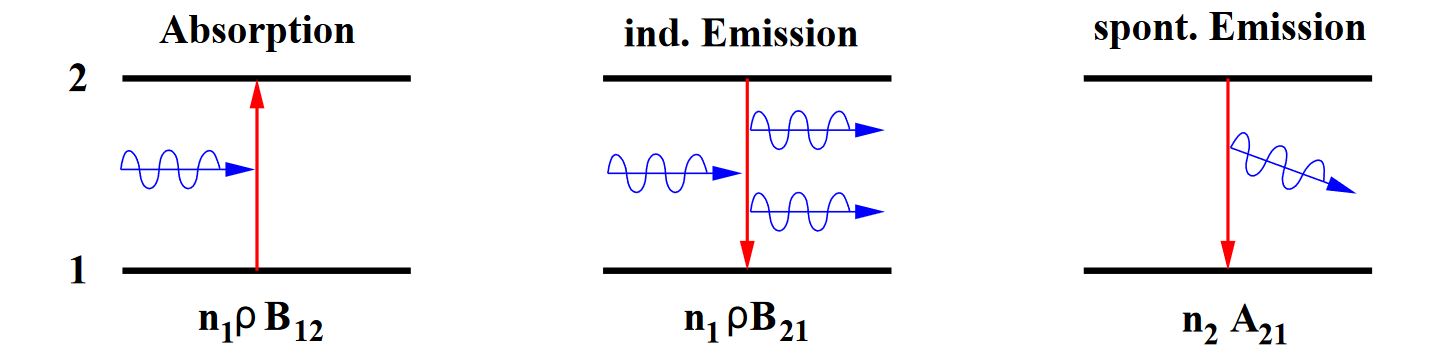
\includegraphics[width=0.75\textwidth]{img/emission.png}
  \caption{Schemata für die Absorption und Emission eines Strahlungsfeldes $\rho(v)$ beieinem 2-Niveau System \cite{FP}}.
  \label{abb:emission}
\end{figure}

Wechselwirkt ein Strahlungsfeldes $\rho(v)$ mit einem Zwei-Niveau-System wird die Besetzungsdichte $n_2$ des angeregten Zustandes durch
spontane sowie durch induzierte Emission verringert und durch Absorption erhöht. Die Anzahl der emittierten bzw. absorbierten folgen

\begin{equation}
\dot{N_A} = n_1 \rho(v) B_12
\end{equation}

\begin{equation}
\dot{N_SE} = n_2 \rho(v) B_21
\end{equation}


\begin{equation}
\dot{N_E} = n_2 A_21
\end{equation}

Wobei die Koeffizien $B_12$, $B_21$ und $A_21$ ein Maß für die Übergangswahrscheinlichkeiten zwischen den Zuständen darstellen.
Hieraus folgen nun folgende Ratengleichungen für die Besetzungsdichten der Niveaus.

\begin{equation}
\frac{d n_1}{dt} = n_1 B_12 \rho + N_2 B_21 \rho + n_2 A_21
\end{equation}

\begin{equation}
\frac{d n_2}{dt} = n_1 B_12 \rho - n_2 B_21 \rho - n_2 A_21
\end{equation}

Im thermischen Gleichgewicht ist der Grundzustand sehr viel stärker besetzt als der angerete Zustand. Um eine Besetzungszahl
Inversion zu erreichen, muss dem Medium sukzessive Energie hinzugefügt werden. Der hier diskutierten Laser nutzt hierfür
den Elektronenstoß. Helium und Neon befinden sich hierfür in einer Glaskapilare mit einer Anode und Kathode. Zwischen Anode und Kathode 
wird eine Spannung von ca. 2 kV angelegt, so dass das Helium mit dem Neon elastisch Stößt und dieses anregt.

\begin{figure}
  \centering
  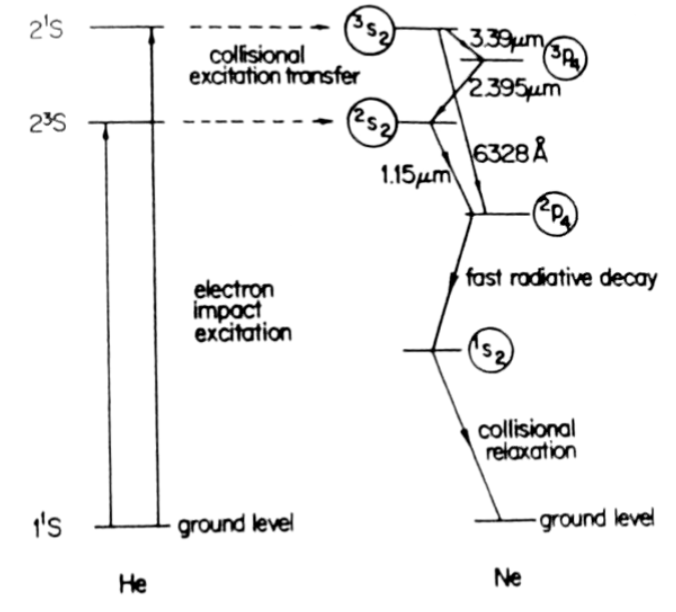
\includegraphics[width=0.75\textwidth]{img/schema.png}
  \caption{Energieniveaus im HeNe-Laser}
  \label{abb:schema}
\end{figure}

Das Energieschema des Lasermaterials definiert die Übergänge und somit auch die Wellenlänge.
Für den HeNe-Laser sind $\lambda = 632.8 \, \text{nm}$ charakteristisch.
Es ist zu beachten, dass die Verstärkung in dem Lasermedium proportional zur zurückgelegten Strecke im Medium ist und einem
exponentiellen Verlauf folgt. Daher erfüllt der Resonator die Aufgabe das Licht möglichst oft durch das aktive Lasermedium
laufen zu lassen und durch sukzessive Verstärkung die Laserschwelle zu errechen. Ein Teil des Lichtes wird an einem der Resonatorspiegel
ausgekoppelt um dieses nutzen zu können.

Der Resonator muss optisch stabil sein, d.h. das in ihm geführte Licht darf den Resonator nicht verlassen. Ein Maß hierfür stellt
die sogenannte Stabilitätsbedingung

\begin{equation}
0 \leq g_1 g_2 < 1
\end{equation}
dar, wobei die Parameter $g_1$ und $g_2$ folgende Form haben:

\begin{equation}
g_i = 1 - \frac{L}{r_i}
\end{equation}


Ferner ist noch zu sagen, dass sich in dem Laserresonator, im Laserbetrieb, longitudinale sowie transversale Moden ausbreiten können.




